% Metrics and decision gates overview
\documentclass[tikz,border=5pt]{standalone}
\usepackage{xcolor}
\usepackage{fontspec}
\usetikzlibrary{arrows.meta,shapes.geometric,fit,shadows.blur,positioning}

% Define color scheme
\definecolor{primaryblue}{RGB}{41,128,185}
\definecolor{secondarygreen}{RGB}{39,174,96}
\definecolor{accentorange}{RGB}{230,126,34}
\definecolor{warningred}{RGB}{231,76,60}
\definecolor{lightgray}{RGB}{236,240,241}
\definecolor{darkgray}{RGB}{52,73,94}
\definecolor{purpleaccent}{RGB}{155,89,182}

\begin{document}
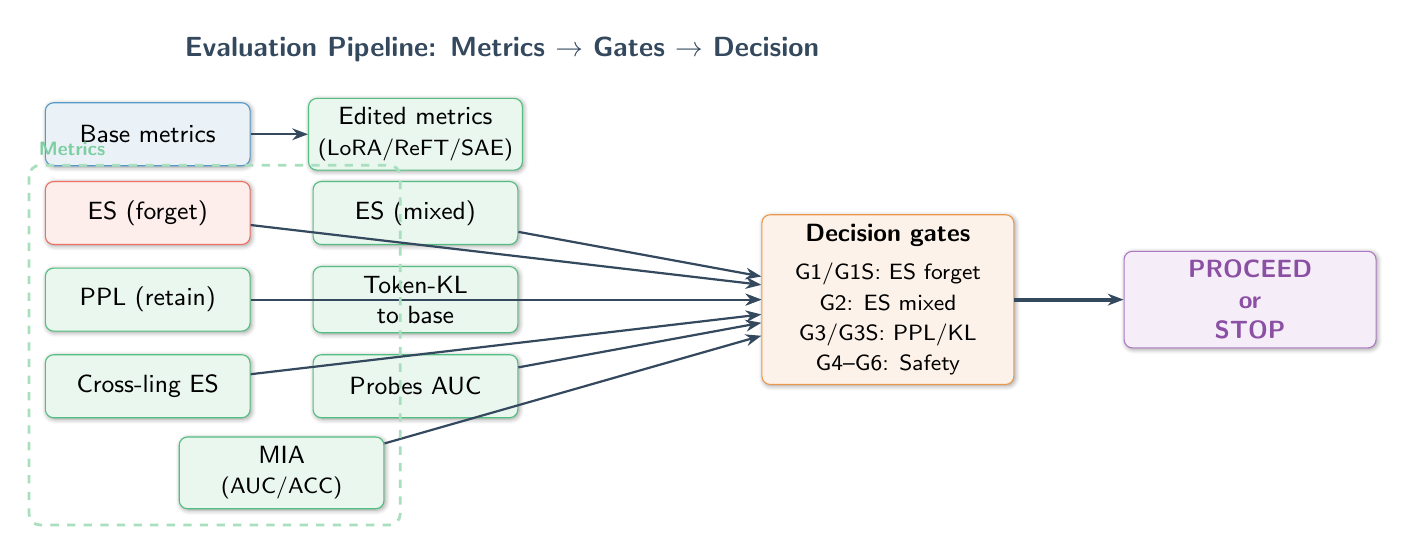
\begin{tikzpicture}[
  node distance=9mm and 12mm,
  block/.style={
    draw=secondarygreen!80,
    fill=secondarygreen!10,
    rounded corners=3pt,
    minimum width=26mm,
    minimum height=8mm,
    align=center,
    font=\sffamily\small,
    blur shadow={shadow blur steps=5, shadow xshift=0.5pt, shadow yshift=-0.5pt}
  },
  baseline/.style={
    draw=primaryblue!80,
    fill=primaryblue!10,
    rounded corners=3pt,
    minimum width=26mm,
    minimum height=8mm,
    align=center,
    font=\sffamily\small,
    blur shadow={shadow blur steps=5, shadow xshift=0.5pt, shadow yshift=-0.5pt}
  },
  gatebox/.style={
    draw=accentorange!80,
    fill=accentorange!10,
    rounded corners=3pt,
    minimum width=32mm,
    minimum height=16mm,
    align=center,
    font=\sffamily\small,
    blur shadow={shadow blur steps=5, shadow xshift=0.5pt, shadow yshift=-0.5pt}
  },
  decision/.style={
    draw=purpleaccent!80,
    fill=purpleaccent!10,
    rounded corners=3pt,
    minimum width=32mm,
    minimum height=10mm,
    align=center,
    font=\sffamily\small\bfseries,
    blur shadow={shadow blur steps=5, shadow xshift=0.5pt, shadow yshift=-0.5pt}
  },
  line/.style={-{Stealth[length=2mm]}, thick, draw=darkgray},
  annot/.style={font=\sffamily\scriptsize, text=darkgray}
]

% Title
\node[anchor=south, font=\sffamily\bfseries, text=darkgray]
  at (45mm,18mm) {Evaluation Pipeline: Metrics $\to$ Gates $\to$ Decision};

% Base and Edited metrics headers
\node[baseline] (base) at (0,10mm) {Base metrics};
\node[block] (arm) at (34mm,10mm) {Edited metrics\\{\footnotesize (LoRA/ReFT/SAE)}};
\draw[line] (base) -- (arm);

% Left column: metrics
\node[block, fill=warningred!10, draw=warningred!80] (esf) at (0,0) {ES (forget)};
\node[block] (esm) at (34mm,0) {ES (mixed)};

\node[block] (ppl) at (0,-11mm) {PPL (retain)};
\node[block] (kl) at (34mm,-11mm) {Token-KL\\to base};

\node[block] (cl) at (0,-22mm) {Cross-ling ES};
\node[block] (pr) at (34mm,-22mm) {Probes AUC};

\node[block] (mia) at (17mm,-33mm) {MIA\\{\footnotesize (AUC/ACC)}};

% Gate box
\node[gatebox] (gate) at (94mm,-11mm) {\textbf{Decision gates}\\[1mm]
  {\footnotesize G1/G1S: ES forget}\\
  {\footnotesize G2: ES mixed}\\
  {\footnotesize G3/G3S: PPL/KL}\\
  {\footnotesize G4--G6: Safety}};

% Decision box
\node[decision, text=purpleaccent!90!black] (dec) at (140mm,-11mm) {PROCEED\\or\\STOP};

% Connect metrics to gate
\draw[line] (esf) -- (gate);
\draw[line] (esm) -- (gate);
\draw[line] (ppl) -- (gate);
\draw[line] (kl) -- (gate);
\draw[line] (cl) -- (gate);
\draw[line] (pr) -- (gate);
\draw[line] (mia) -- (gate);

% Connect gate to decision
\draw[line, line width=1.5pt] (gate) -- (dec);

% Add grouping boxes
\draw[draw=secondarygreen!40, line width=1pt, rounded corners, dashed]
  ($(esf.north west)+(-2mm,2mm)$) rectangle ($(mia.south east)+(2mm,-2mm)$);
\node[anchor=south west, font=\sffamily\scriptsize\bfseries, text=secondarygreen!60]
  at ($(esf.north west)+(-2mm,2mm)$) {Metrics};

\end{tikzpicture}
\end{document}
